% -*- mode: fundamental -*-

% ****************************************************************

\chapter{RISC-V: the Drum unpipelined CPU (using Rules instead of {\tt StmtFSM})}

\markboth{Ch \arabic{chapter}: The Drum CPU with Rules}{\copyrightnotice}

\setcounter{page}{1}
% \renewcommand{\thepage}{\arabic{page}}
\renewcommand{\thepage}{\arabic{chapter}-\arabic{page}}

\label{ch_Drum_Rules}

% ****************************************************************

% ----------------
\vspace{2ex}

\centerline{
\includegraphics[width=1in,angle=0]{Figures/Fig_Under_Construction}}

\vspace{2ex}
% ----------------

\section{Introduction}

In this chapter we use show a manual translation of The Drum CPU
behavior was shown using BSV's \verb|StmtFSM| construct in
Section~\ref{Sec_Drum_CPU_module_behavior}.  Here we show a manual
translation of the FSM into Rules, to reinforce the idea that
\verb|StmtFSM| is just a convenient, higher-level view of rules;
\verb|StmtFSM| does not add any genuine new semantic power to BSV.

construct.
\begin{figure}[htbp]
  \centerline{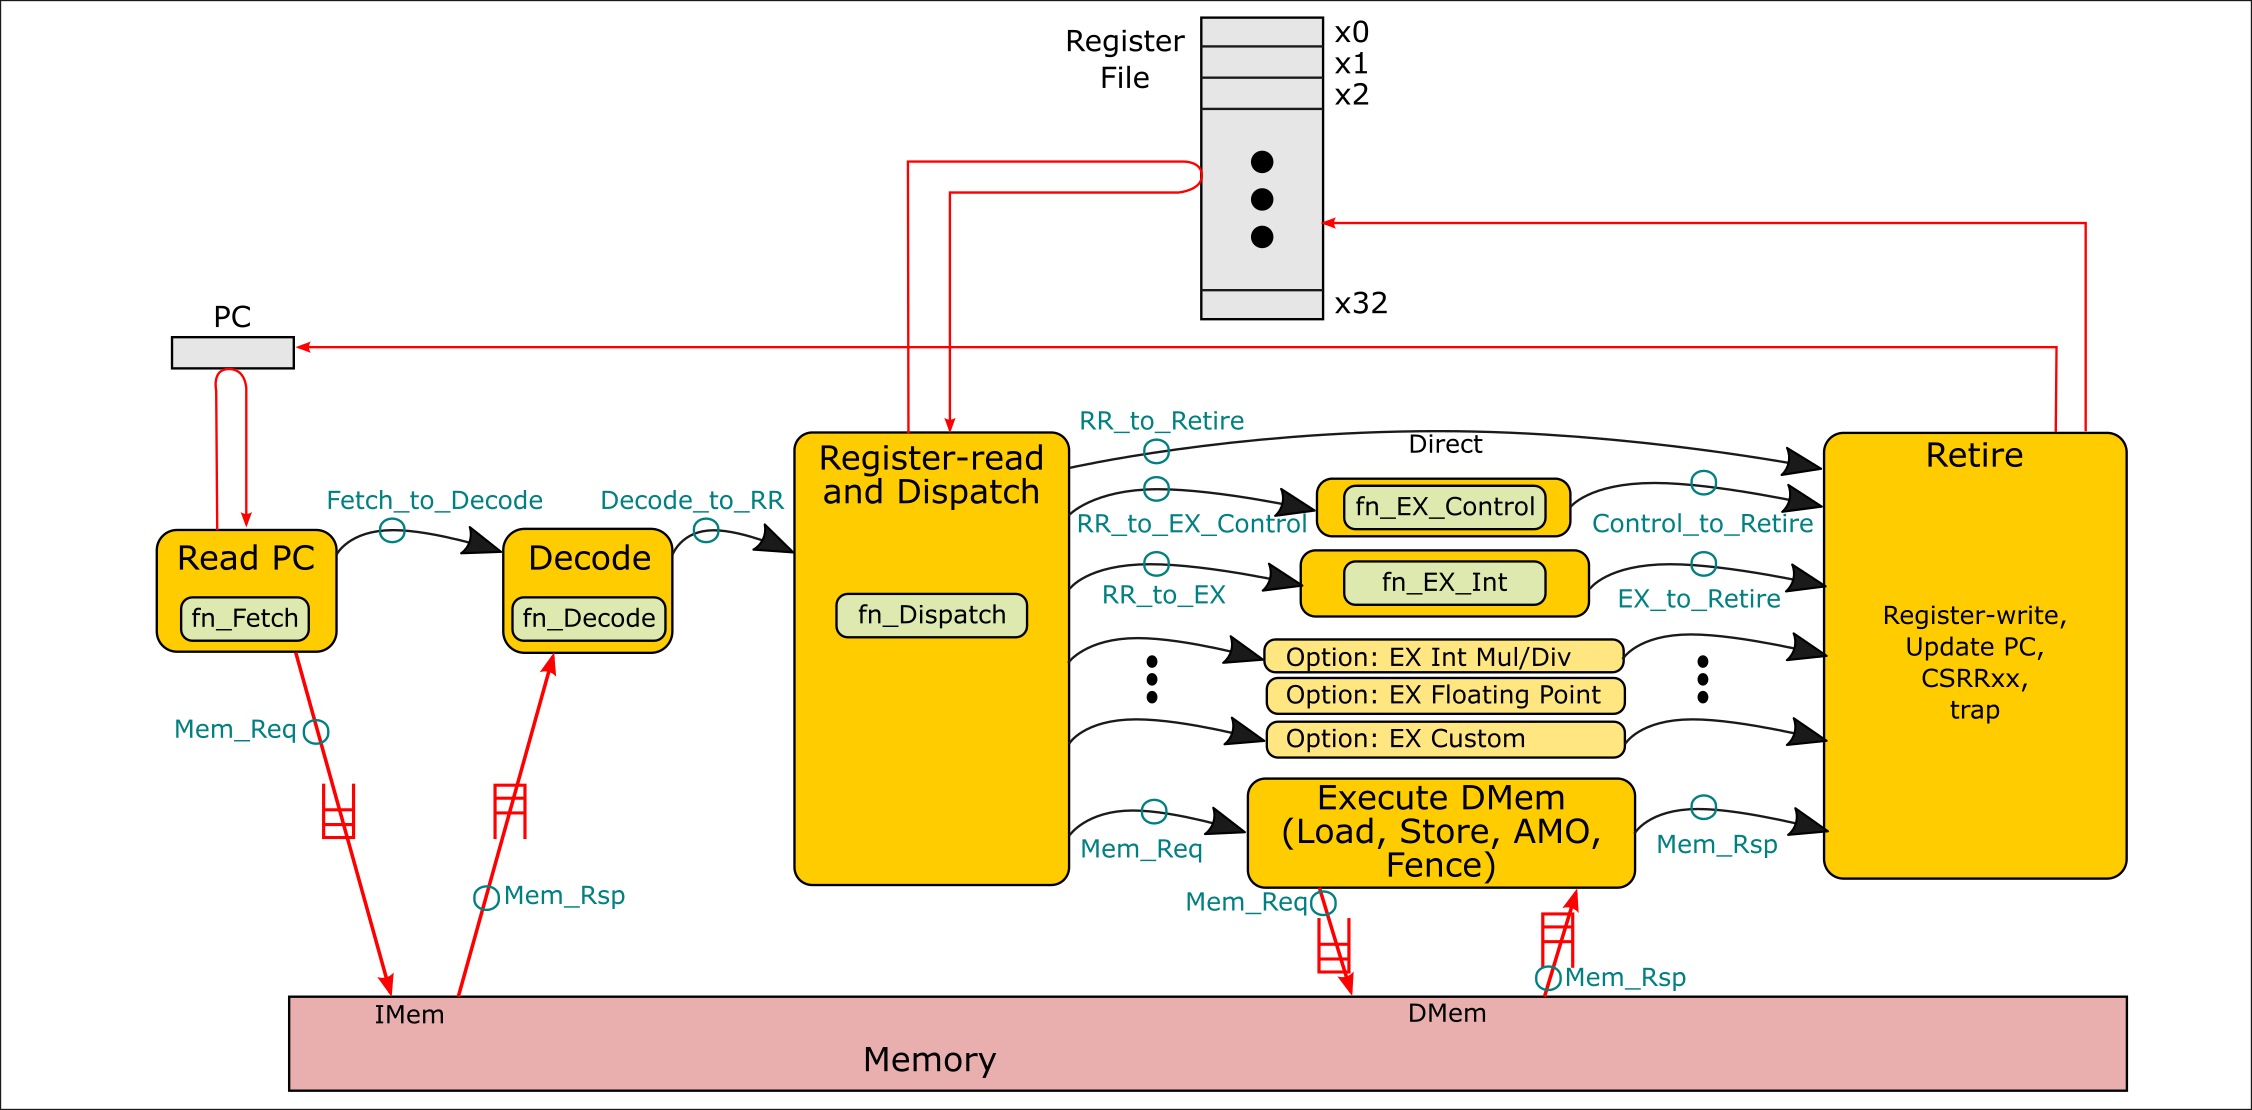
\includegraphics[width=6in,angle=0]{Figures/Fig_Instr_Exec_w_structs}}
  \caption{\label{Fig_Drum_II_Instr_Exec}
           Simple interpretation of RISC-V instructions
	   (same as Fig.~\ref{Fig_Simple_Instr_Exec_w_structs})}
\end{figure}

% ****************************************************************

\section{The Drum CPU module behavior}

% ****************************************************************

\section{Conclusion}

And that is the complete Drum CPU!

% ****************************************************************
